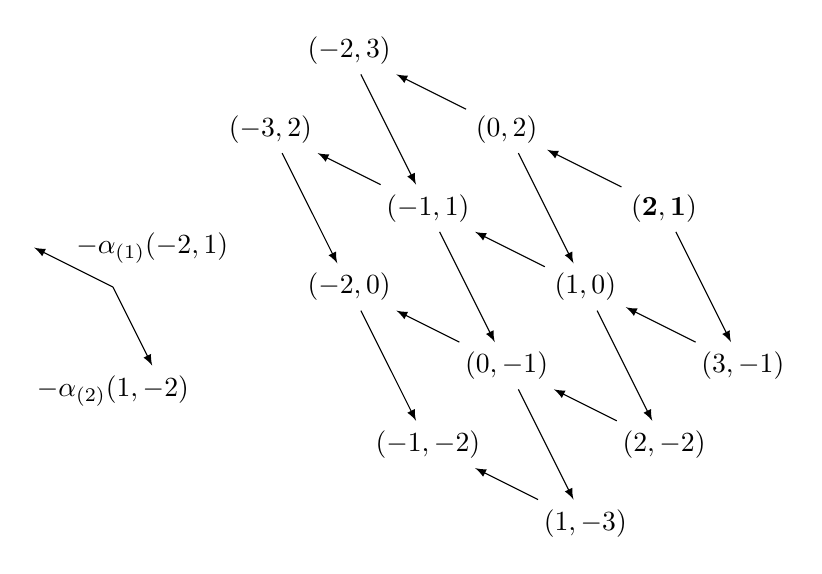
\begin{tikzpicture}


\draw [-latex] (-5,0) -- (-4.5,-1);
\draw [-latex] (-5,0) -- (-6,0.5);
\node [below] at (-5,-1) {$ -\alpha_{(2)} \rightsquigarrow (1,-2)$};
\node at (-4.5,0.5) {$-\alpha_{(1)} \rightsquigarrow (-2,1)$};



\node (v12) at (2,1) {$\mathbf{(2,1)}$};
\node (v13) at (3,-1) {$(3,-1)$};
\draw [-latex] (v12) edge (v13);
\node (v15) at (0,2) {$(0,2)$};
\node (v16) at (-2,3) {$(-2,3)$};
\draw [-latex] (v12) edge (v15);
\draw [-latex] (v15) edge (v16);
\node (v14) at (1,0) {$(1,0)$};
\node (v17) at (2,-2) {$(2,-2)$};
\draw [-latex] (v15) edge (v14);
\draw [-latex] (v14) edge (v17);
\node (v18) at (-1,1) {$(-1,1)$};
\node (v19) at (0,-1) {$(0,-1)$};
\node (v20) at (1,-3) {$(1,-3)$};
\draw [-latex] (v16) edge (v18);
\draw [-latex] (v18) edge (v19);
\draw [-latex] (v19) edge (v20);
\node (v21) at (-1,-2) {$(-1,-2)$};
\draw [-latex] (v20) edge (v21);
\draw [-latex] (v17) edge (v19);
\draw [-latex] (v14) edge (v18);
\node (v22) at (-2,0) {$(-2,0)$};
\draw [-latex] (v19) edge (v22);
\draw [-latex] (v13) edge (v14);
\node (v23) at (-3,2) {$(-3,2)$};
\draw [-latex] (v18) edge (v23);
\draw [-latex] (v23) edge (v22);
\draw [-latex] (v22) edge (v21);
\end{tikzpicture}